\documentclass[acmtog]{acmart}
\usepackage{graphicx}
\usepackage{subfigure}
\usepackage{natbib}
\usepackage{listings}
\usepackage{bm}

\definecolor{blve}{rgb}{0.3372549 , 0.61176471, 0.83921569}
\definecolor{gr33n}{rgb}{0.29019608, 0.7372549, 0.64705882}
\makeatletter
\lst@InstallKeywords k{class}{classstyle}\slshape{classstyle}{}ld
\makeatother
\lstset{language=C++,
	basicstyle=\small\ttfamily,
	keywordstyle=\color{blve}\ttfamily,
	stringstyle=\color{red}\ttfamily,
	commentstyle=\color{magenta}\ttfamily,
	morecomment=[l][\color{magenta}]{\#},
	classstyle = \bfseries\color{gr33n},
	breaklines=true, 
	tabsize=2
}
\lstset{basicstyle=\ttfamily}

% Title portion
\title{Assignment 3:\\ {Ray Tracing with Direct Lighting}} 

\author{Name:\quad Yang Hongdi  \\  student number:\ 2019533234
\\email:\quad yanghd@shanghaitech.edu.cn}

% Document starts
\begin{document}
\maketitle

\vspace*{2 ex}

\section{Introduction}
In this project, simple Ray tracing with Direct lighting is performed. Phong lighting model is used for radiance calculation. Anti-aliasing is performed with rotated grid pattern. 
Some textures have been added to the Boxes with normal mapping.

\section{Implementation Details}
\subsection{Pin-hole camera model}
First, we construct axes for camera coordinate system by using lookat point and reference up direction.
\begin{lstlisting}
void Camera::lookAt(const vec3 &lookAt, const vec3 &refUp) {
	this->forward = (position - lookAt).normalized();
	this->right = refUp.cross(forward).normalized();
	this->up = forward.cross(right).normalized();
	this->halfFovScale = tan(radians(verticalFov * 0.5f));
}
\end{lstlisting}
Then we can generate ray from camera for a specified pixel.
\begin{figure}[H]
	\centering
	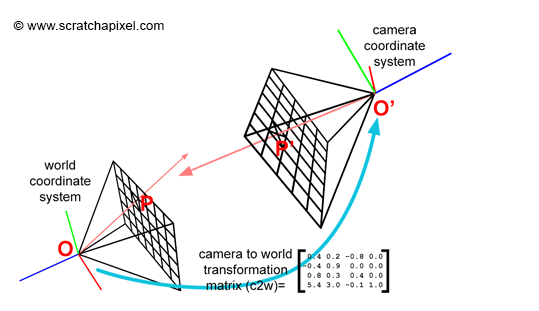
\includegraphics[width=0.4\textwidth,height=2in]{camera.png}
	\caption{world space coordinate calculation}
\end{figure}
\begin{figure}[H]
	\centering
	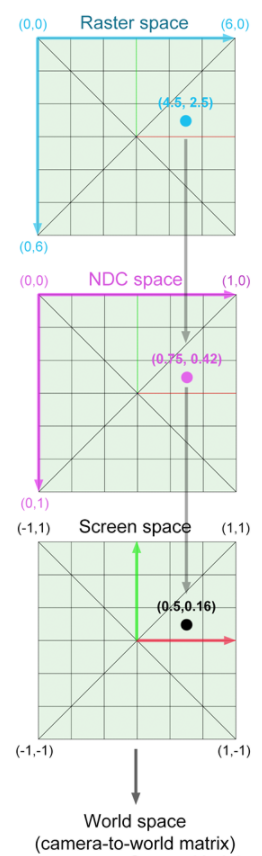
\includegraphics[width=0.3\textwidth,height=4.5in]{transform.png}
	\caption{coordinate transform}
\end{figure}
As the image shows, we already have the camera coordinate system, by simply transforming the pixel coordinate in raster space to coordinate in screen space, 
then we can easily compute its position in world space.\\
Then we shoot a ray from the camera position to pixel position, and we set its origin as the pixel position and the direction as $norm(P_{pixel} - P_{camera})$
\begin{lstlisting}
Ray Camera::generateRay(Float dx, Float dy) const {
	vec3 position;
	vec3 dir;

	Float width = film.resolution.x();
	Float height = film.resolution.y();
	Float screen_x, screen_y;
	screen_x = (2 * (dx)/width - 1) * film.getAspectRatio() * halfFovScale * focalLength;
	screen_y = (2 * (dy)/height - 1) * halfFovScale * focalLength;
	vec3 screenCenter = this->position - focalLength * forward;
	position = screenCenter + screen_x * right + screen_y * up;
	dir = (position - this->position).normalized();

return Ray{position, dir};
}
\end{lstlisting}

\subsection{Ray-triangle intersection test}
To test if the ray intersects with the triangle, we adopt Moller-Turmbore instersection algorithm.\\
First, we know the ray's parametric equation :
$$P = O + tD$$
And we can denot any point in the triangle as :
$$P = (1- u - v)A + uB + uC$$
so we have :
$$O + tD = (1- u - v)A + uB + uC$$
by some transformation :
$$\left[\begin{matrix}
	-D & (B-A) & (C-A)
\end{matrix}\right]\left[\begin{matrix}
	t \\ u \\ v
\end{matrix}\right] = O - A$$
We denote $T = O - A, E_1 = B - A$ and $E_2 = C - A$, applying Cramer's rule and determinant property, we get :
$$\left[\begin{matrix}
	t \\ u \\ v
\end{matrix}\right] = \frac{1}{P \cdot E_1}\left[\begin{matrix}
	Q \cdot E_2 \\ P \cdot T \\ Q	\cdot D
\end{matrix}\right]$$
where $P = D \times E_2$ and $D = T \times E_1$. Now we can easily compute $t,u,v$
Here are the code.
\begin{lstlisting}
bool Triangle::intersect(Interaction &interaction, const Ray &ray) const {
	const vec3 &v0 = mesh->p[v[0]];
	const vec3 &v1 = mesh->p[v[1]];
	const vec3 &v2 = mesh->p[v[2]];
	
	vec3 E1 = v1 - v0;
	vec3 E2 = v2 - v0;
	vec3 T = ray.origin - v0;

	vec3 P = ray.direction.cross(E2);
	vec3 Q = T.cross(E1);
	Float det = P.dot(E1);
	if (abs(det) < SHADOW_EPS) return false;
	vec3 tuv = 1/(P.dot(E1)) * vec3(Q.dot(E2), P.dot(T), Q.dot(ray.direction));
	Float t = tuv.x();
	Float u = tuv.y();
	Float v = tuv.z();
	...
}
\end{lstlisting}
And when $t \geq 0, u \geq 0, v \geq 0, 1 - u -v \geq 0$, the ray intersects with the triangle.
\subsection{Area Light}
For area light, we just uniformly sample some point lights on it. And for every point light, the radiance
will be $\frac{L}{N}$, where $N$ is the number of samples.
\subsection{Phong lighting integrator}
To calculate the irrandiance, we use phong lighting model. Basically we have following steps :
\begin{enumerate}
	\item [1.] For each ray, we check how it intersects with the scene.
	\begin{itemize}
		\item If the ray intersects with nothing, return (0,0,0).
		\item If the ray intersects with light, return light's color.
		\item If the ray intersects with geometry, go to step 2.
	\end{itemize}
	\item [2.] We shoot another ray from the intersection point to one light sample.
	\begin{itemize}
		\item If the ray is blocked by other objects, we only add ambient light.
		\item If the ray only intersects with the light, we  calculate the phong lighting on that point.
	\end{itemize}
	\item [3.] We repeat step2 for every light sample on area light.
\end{enumerate}
Then we have the irrandiance, here are the code.
\begin{lstlisting}
vec3 PhongLightingIntegrator::radiance(Scene &scene,
						const Interaction &interaction,
						const Ray &ray) const {
	if (interaction.type == interaction.NONE)
	{
		return vec3::Zero();
	}
	else if (interaction.type == interaction.LIGHT)
	{
		return scene.getLight()->getColor();
	}
	else if (interaction.type == interaction.GEOMETRY)
	{
		vec3 ambient = (scene.getAmbientLight().array() * interaction.lightingModel.ambient.array()).matrix();
		vec3 diffuse = vec3::Zero();
		vec3 specular = vec3::Zero();
		for (LightSamplePair pointLight : scene.getLight()->samples())
		{
			///Diffuse
			vec3 lightDir = (pointLight.first - interaction.entryPoint).normalized();
			Ray lightRay(interaction.entryPoint, lightDir);
			if (!scene.isShadowed(lightRay))
			{
				///Diffuse
				Float diff = std::max(interaction.normal.dot(lightDir), 0.0f);
				Eigen::Array3f temp_diff = diff * pointLight.second.array() * interaction.lightingModel.diffusion.array();
				diffuse += temp_diff.matrix();

				///Specluar
				vec3 reflectDir = (2 * lightDir.dot(interaction.normal) * interaction.normal - lightDir).normalized();
				Float spec = (Float)std::pow(std::max(reflectDir.dot(-ray.direction), 0.0f), interaction.lightingModel.shininess);
				Eigen::Array3f temp_spec =  spec * pointLight.second.array() * interaction.lightingModel.specular.array();
				specular += temp_spec.matrix();
			}
		}
		return ambient + diffuse + specular;
	}
	return vec3::Zero();
}
\end{lstlisting}
To render the scene, we just apply the function on every pixel.

\subsection{Anti aliasing}
For anti aliasing, rotated grid is used for sampling in pixel.\\
\begin{figure}[H]
	\centering
	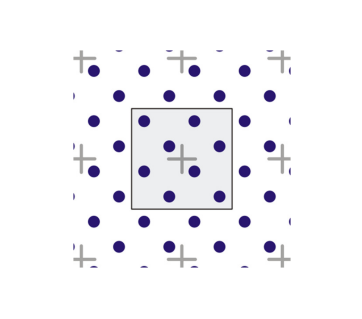
\includegraphics[width=0.4\textwidth,height=2in]{antialiasing.png}
	\caption{Rotated grid}
\end{figure}
To perform anti aliasing and also for time effiency, we sample 4 points in each pixel with a rotation of $26.6^{\circ}$.

\subsection{Texture}
Texture with normal mapping is performed. As in section 2.2 Ray-triangle intersection test, we have $u, v$. So we simply load the color on pixel
$(int)\frac{u}{width}, (int)\frac{v}{height}$ on the Texture map.
\begin{lstlisting}
vec3 Texture::getColor(vec2 uv) const
{
	int x = (int) (uv.x() * width);
	int y = (int) (uv.y() * height);
	x = (x == width) ? x - 1 : x;
	y = (y == height) ? y - 1 : y;
	return color_data[x + y * width];
}
\end{lstlisting}

\section{Results}
\begin{figure}[H]
    \centering
    
    \subfigure[Scene0 with no Msaa]{
    \begin{minipage}[t]{0.45\linewidth}
    \centering
    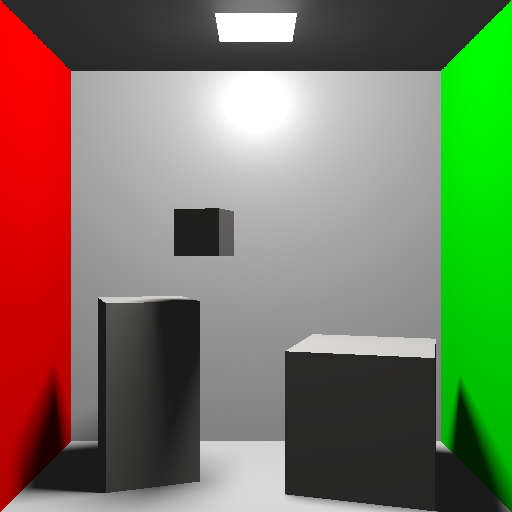
\includegraphics[width=1.5in]{output_nomsaa.png}
    %\caption{original image}
    \end{minipage}%
    } \quad \quad
    \subfigure[Scene0]{
    \begin{minipage}[t]{0.45\linewidth}
    \centering
    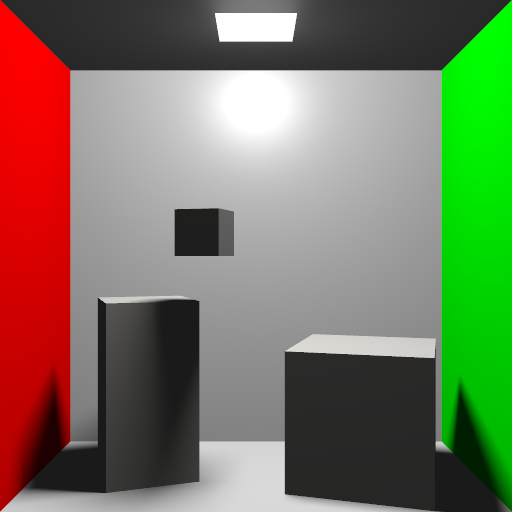
\includegraphics[width=1.5in]{output_scene0.png}
    %\caption{ground truth}
    \end{minipage}%
    }%
                    
    \subfigure[Scene1]{
    \begin{minipage}[t]{0.45\linewidth}
    \centering
    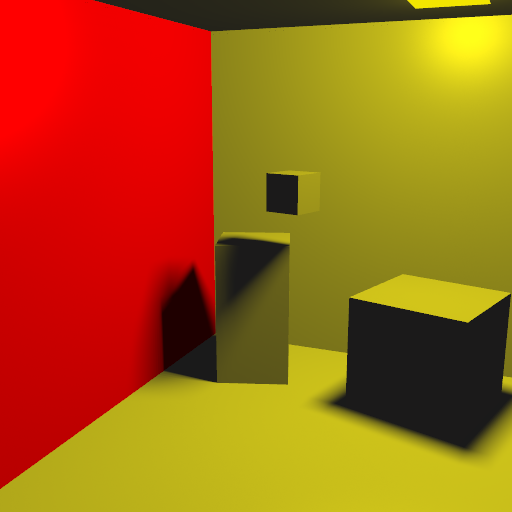
\includegraphics[width=1.5in]{output_scene1.png}
    %\caption{depth prediction result}
    \end{minipage}
    }

    \subfigure[Scene2]{
    \begin{minipage}[t]{0.45\linewidth}
    \centering
    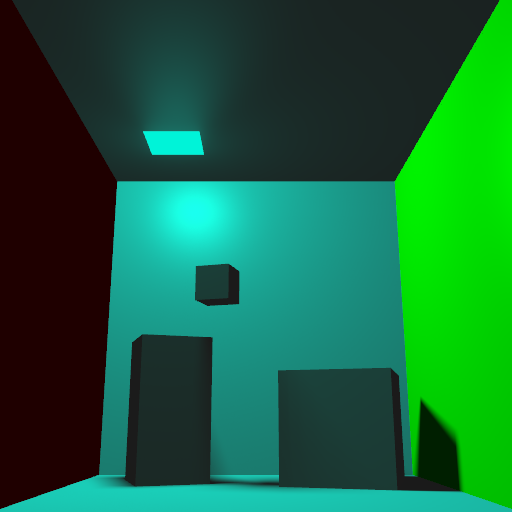
\includegraphics[width=1.5in]{output_scene2.png}
    %\caption{original image}
    \end{minipage}%
    } \quad \quad
    \subfigure[Scene0 with texture]{
    \begin{minipage}[t]{0.45\linewidth}
    \centering
    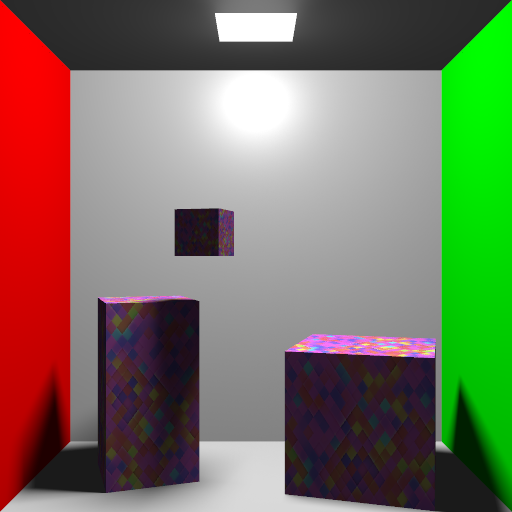
\includegraphics[width=1.5in]{output_scene0_texture.png}
    %\caption{ground truth}
    \end{minipage}%
    }%
    \subfigure[Scene0 with normal mapping]{
    \begin{minipage}[t]{0.45\linewidth}
    \centering
    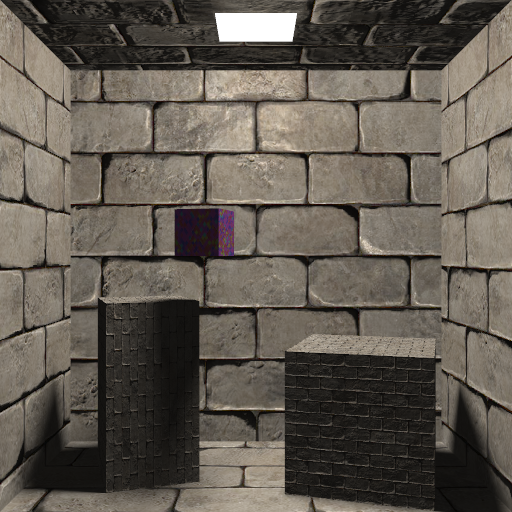
\includegraphics[width=1.5in]{output_normal.png}
    %\caption{ground truth}
    \end{minipage}%
    }%
    \centering
    \caption{Result}
    \end{figure}
\end{document}
